\documentclass{article}
\usepackage[utf8]{inputenc}
\usepackage{amsmath}
\usepackage{amsfonts}
\usepackage{amsthm}
\usepackage{amssymb}
\usepackage{graphicx}
\usepackage{float}
\usepackage[margin=0.75in]{geometry}
\usepackage{xcolor}
\usepackage[makeroom]{cancel}
\usepackage{caption}
\usepackage{subcaption}
\usepackage{mwe}
% adds indent to first paragraph after section tag
\usepackage{indentfirst}
\theoremstyle{remark}
\newtheorem*{remark}{Remark}
% add tab command to file
\newcommand\tab[1][1cm]{\hspace*{#1}}
\newcommand{\R}{\mathbb{R}}
\newcommand{\N}{\mathbb{N}}
\newcommand{\norm}[1]{\left\lVert#1\right\rVert}
\DeclareMathOperator{\Tr}{Tr}
\DeclareMathOperator{\spn}{span}
\title{Final Report: Reversible Architectures for Arbitrarily Deep Residual Neural Networks \\ \large Course 049064: Variational Methods in Image Processing}
\author{\small Jonathan Masin \& Netanel Rothschild}
\begin{document}
% remove date from title
\date{}
\maketitle
\section*{Background}
    Deep Residual Networks as of recently have been pushing state-of-the-art performance tasks with deeper and wider architectures. This paper 
has set out to interpret Deep Residual Networks as ordinary differential equations (ODEs). The motivation behind this, is the fact that 
ODEs have long been studied in mathematics and physics with rich theoretical and empirical success. Using this interpretation, the authors 
developed a theoretical framework on stability and reversibility of deep neural networks, the paper outlines three reversible neural network 
architectures that may go arbitrarily deep in theory. \par 
    The backbone of this paper is in proving the reversibility of the networks, which in turn allow for memory-efficient implementations, 
as they have no need to store the activation functions for most of the layers \par 
    The paper goes into detail of the theoretical background (which we will cover in this section) and demonstrates examples of experiments 
done, which we will replicate and improve on. Datasets used in the experiments are CIFAR-10, CIFAR-100, and STL-10. With baseline architectures 
used as comparisons. A major strength of the paper's implementation is that the models built using the theoretical background out perform 
strong baseline models, over fewer training data. \par 
    The authors claim the problem with Residual Networks is that, although widely used, there exist little theoretical analysis and guidelines for 
designing and training ResNets. This can be solved by viewing ResNets as ODEs as follows:
%2 images per row
\begin{figure}[H]
    \centering
    \begin{minipage}{0.45\textwidth}
        \centering
        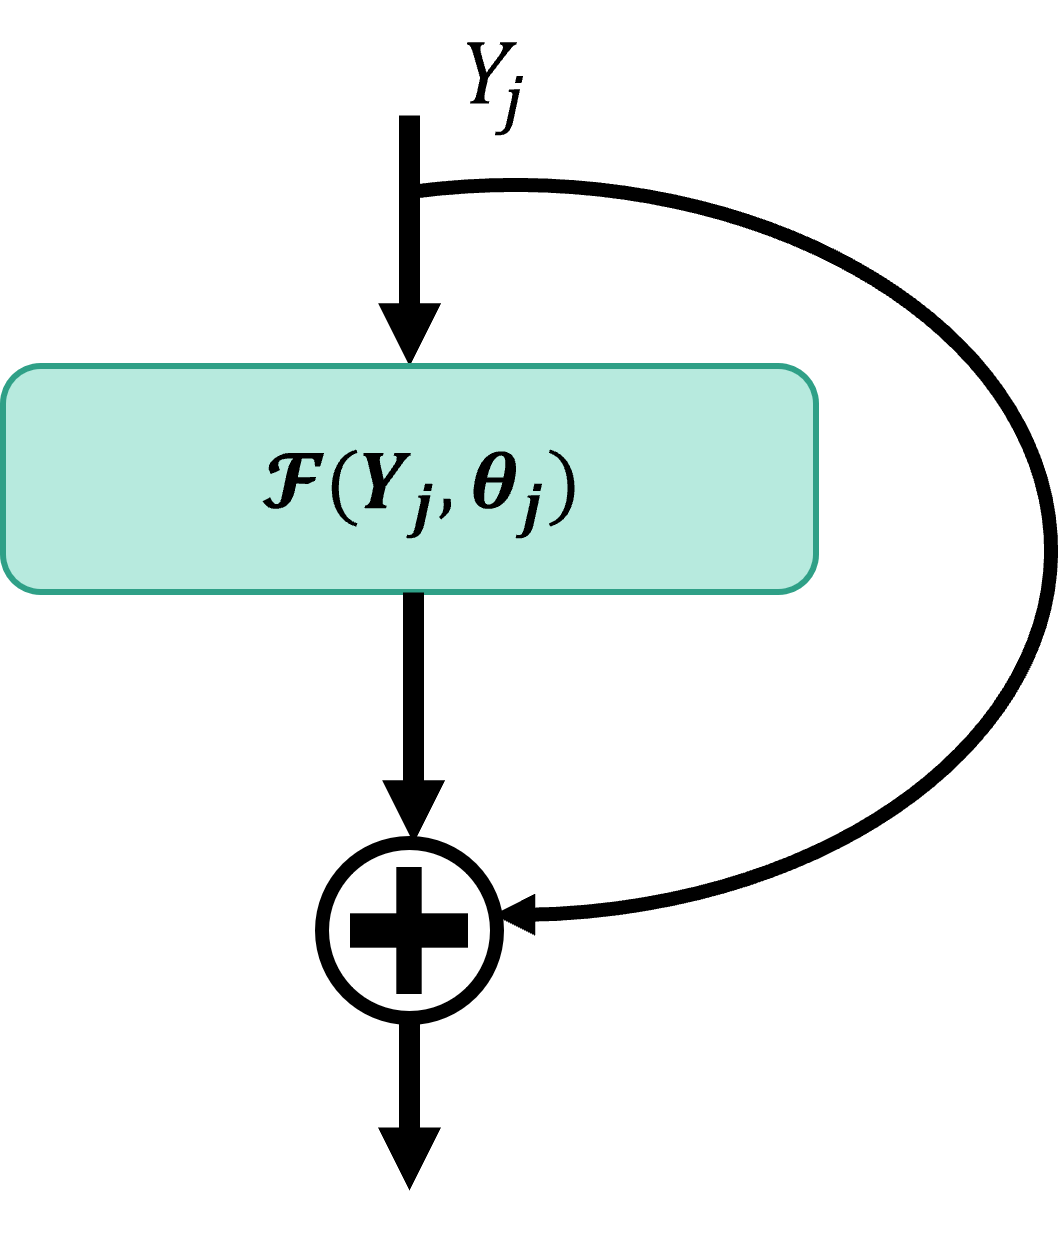
\includegraphics[scale=0.5]{imgs/residual_block.png} % first figure itself
        \caption{residual block}
    \end{minipage}\hfill
    \begin{minipage}{0.45\textwidth}
        \centering
        Output of block:
        \begin{gather*}
            Y_{j+1} = Y_j + \mathcal{F}(Y_j, \theta_j) \\
            \text{multiply by $h$} \\
            Y_{j+1} = Y_j + h\mathcal{F}(Y_j, \theta_j) \rightarrow \\
            \mathcal{F}(Y_j, \theta_j) = \frac{Y_{j+1} - Y_j}{h} \\
            \xrightarrow[]{h \rightarrow 0} \dot{Y}(t) = \mathcal{F}(Y(t), \theta(t)); Y(0) = Y_0
        \end{gather*}
    \end{minipage}
\end{figure}

\par 
    A important definition to outline is "Reversibility", as it is the key element which allows for memory efficient implementations.\\
\textit{Definition Reversibility: An architecture is reversible if it allows the reconstruction of the activations going from the end to the beginning.}

\begin{figure}[H]
    \centering
    \begin{minipage}{0.45\textwidth}
        \centering
        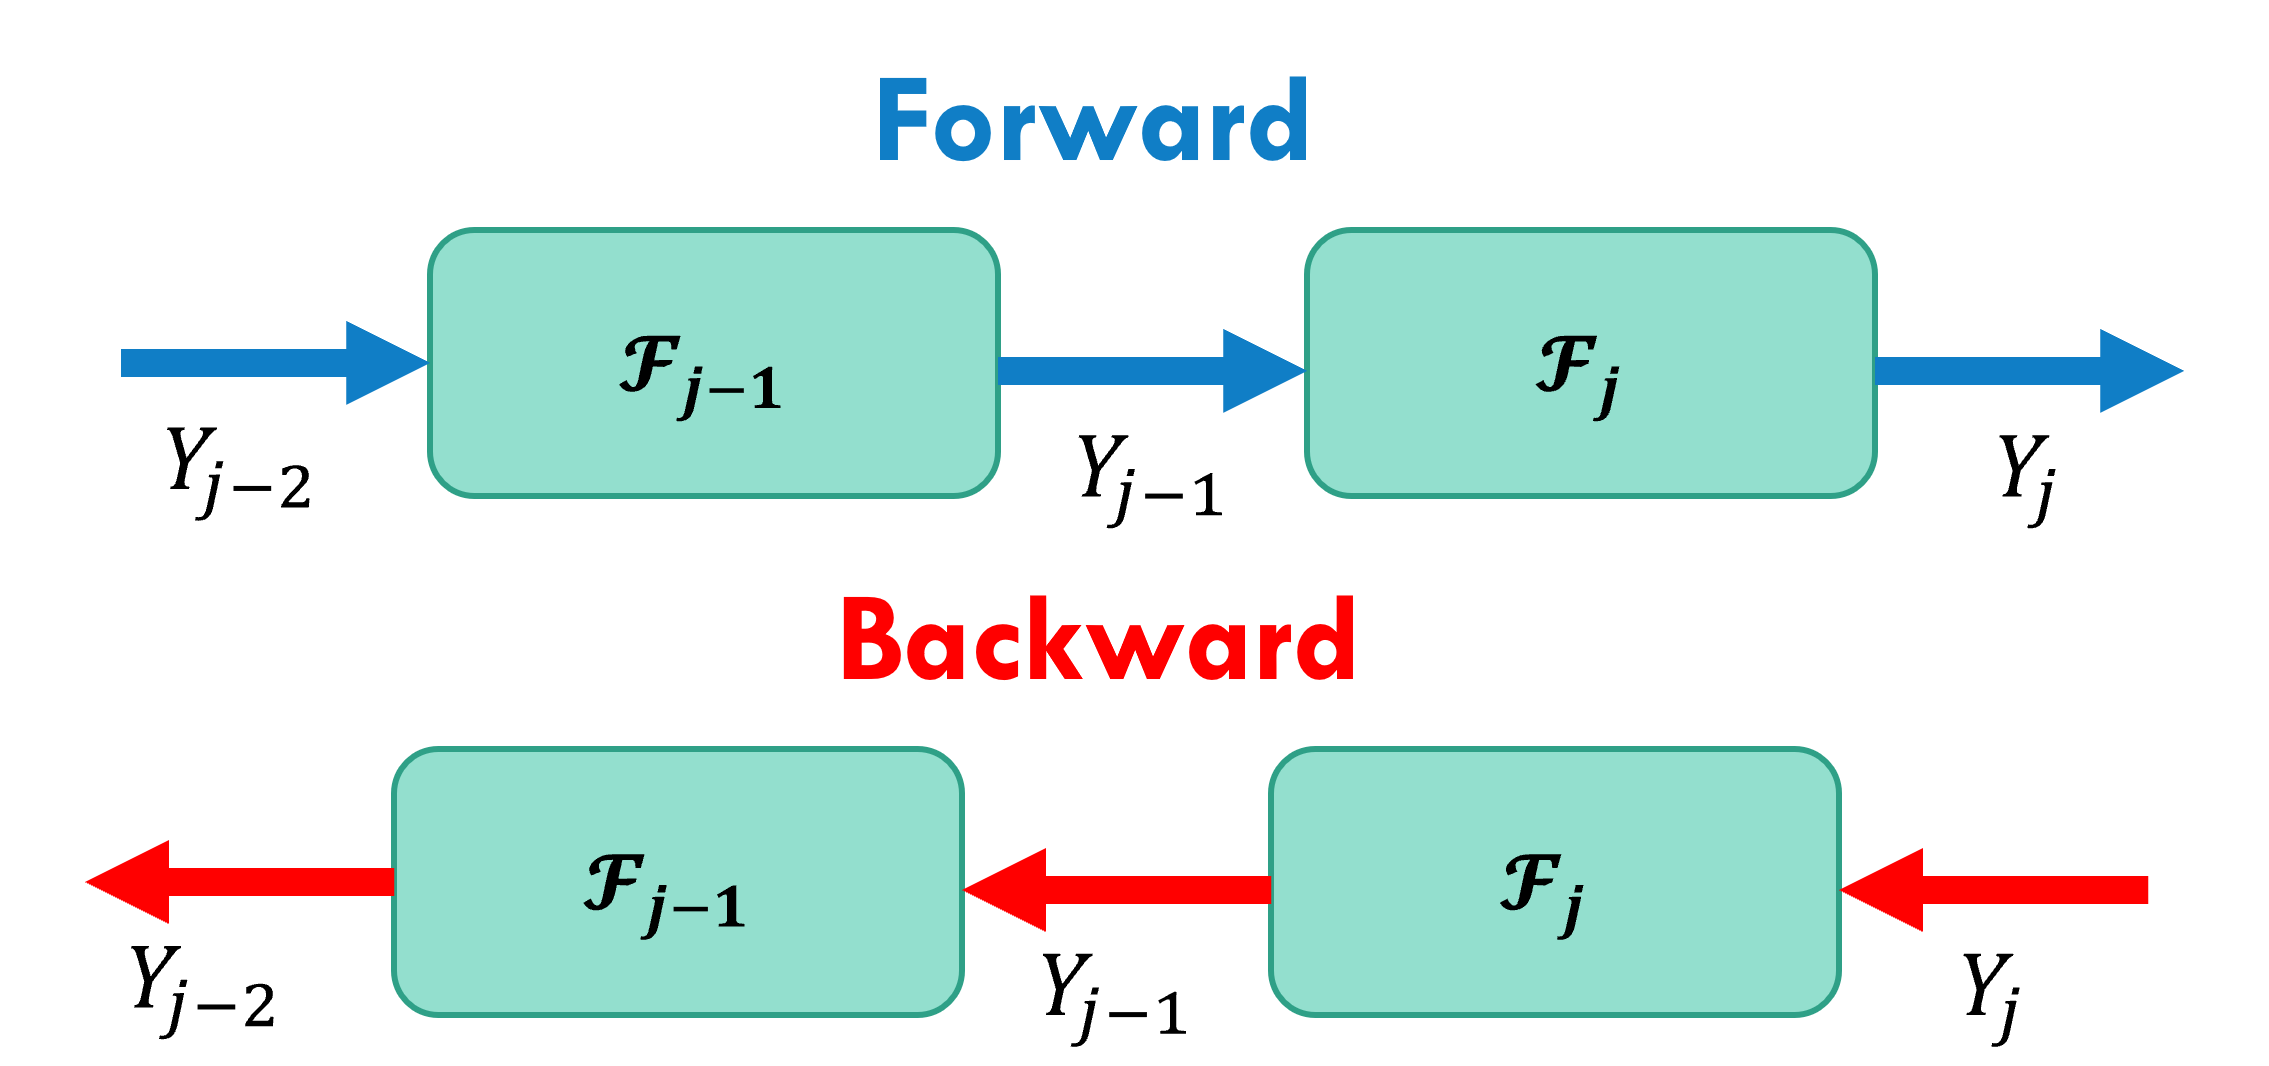
\includegraphics[scale=0.5]{imgs/revesibility_chart.png} % first figure itself
        \caption{forward and backward diagram}
    \end{minipage}\hfill
    \begin{minipage}{0.45\textwidth}
        \centering
        A network is reversible if for:
        \begin{gather*}
            Y_{j-2} = \mathcal{F}^{-1}_{j-1}(\mathcal{F}^{-1}_{j}(\dots \mathcal{F}^{-1}_{N}(Y_N)))\\
            Y_j = \mathcal{F}_{j}(\mathcal{F}_{j-1}(\dots \mathcal{F}_{N}(Y_0))) \\
            \mathcal{F}^{-1}_{k} \text{ Exists } \forall k \Rightarrow \text{Architecture is Reversible}
        \end{gather*}
    \end{minipage}
\end{figure}

Understanding how reversibility allows for a memory efficient implementations will be explained through an example further under the Section "Single Problem"

\end{document}
